\subsection{Section 4.1}
\label{sec:noson-section-4-1}

\subsubsection{Equation (4.5)}
\label{sec:noson-equation-4-5}

I would like to thank \href{http://lattes.cnpq.br/0162506805992681}{
    Victor Santos de Souza
}
for reviewing this section and helping me to keep on the rails of
the mathematical and physical formalisms.

The value $|c_i|^2$ is divided by $|\ket\psi|^2$ because
there is no assumption that $\ket\psi$ is unitary.
This division guarantees that the probabilities sum up to $1$
($\sum_i |c_i|^2 = 1$).

More interesting, from this equation it is possible to deduce that
by multiplying a state $\ket\psi = \sum_i c_i \ket{x_i}$ by
any complex number $z \neq 0$ does not change it
because the measurement probabilities proportion is maintained.

To conclude this, assume that $\ket\psi = \sum_i c_i \ket{x_i}$, and
$\ket\varphi = z \ket\psi = \sum_i d_i \ket{x_i} = \sum_i c_i \ket{y_i}$,
where $\forall i (c_i, d_i, z \in \mathbb{C} \land
d_i = z c_i \land \ket{y_i} = z \ket{x_i})$ -
$\land$ denotes the logical and.
Then prove that $\forall i, p(y_i) = p(x_i)$,

\begin{align}
    p(y_i) &= \frac{|d_i|^2}{|\ket\varphi|^2}
        = \frac{|d_i|^2}{\sum_j|d_j|^2}
        = \frac{|z c_i|^2}{\sum_j|z c_j|^2} 
        \\[5pt]
        &= \frac{|z|^2 |c_i|^2}{\sum_j|z|^2 |c_j|^2}
        = \frac{|z|^2 |c_i|^2}{|z|^2 \sum_j |c_j|^2}
        \\[5pt]
        &= \frac{|c_i|^2}{\sum_j |c_j|^2}
        = p(x_i) .
\end{align}

Due to the particle-wave duality,
it may be interesting to visualise this result in a graph.
Let a state be interpreted as a wave until the end of this section.
Therefore, there exists a corresponding graph to the wave.
Suppose $\ket \psi = \sum_i c_i \ket{x_i}$,
where $c_i \in \mathbb{C}$ and $\ket{x_i} \in \mathbb{C}^n$ form an orthonnormal basis.
It is known that a linear product can be defined as a function
from two vectors to a complex number
($\mathbb{C}^n \times \mathbb{C}^n \rightarrow \mathbb{C}$).
Therefore, it is possible to define $\psi(x)$ as a function that calculates $\braket x \psi$
(the projection of $\ket \psi$ along $\ket x$) where $\ket x \in \set{\ket{x_i}}$).
Analogously, for $\ket \varphi = \sum_i c_i \ket{x_i}$, define
$\varphi(x) = \braket x \varphi$.
Similarly, it is also admissible to image $\psi(x)$ and $\varphi(x)$ as a functions that
map the $\ket x$ domain to complex numbers ($\mathbb{C}^n \rightarrow \mathbb{C}$).
It is interesting to interpret the linear product as a function because
it is possible to calculate probabilites by using integration,
similarly to what is done in statistics
($\braket \psi \varphi = \int dx \braket \psi x \braket x \varphi$).

\begin{figure}[htb]
    \centering
    \begin{subfigure}[b]{0.45\textwidth}
        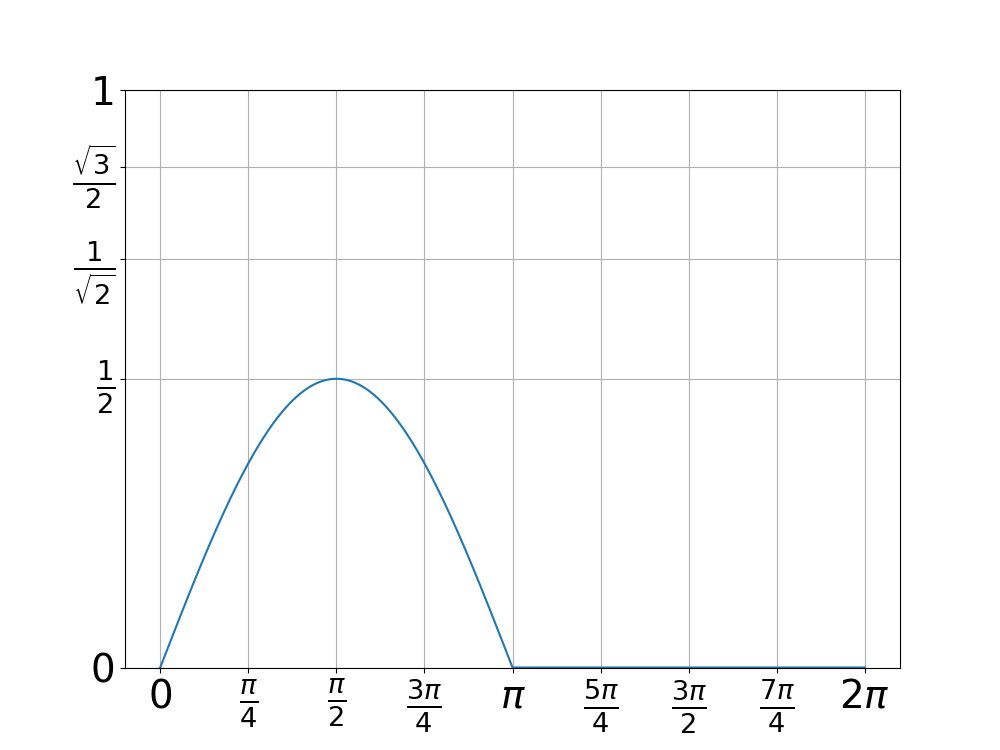
\includegraphics[width=\textwidth]{img/noson/chapter04/section4_1/psi.png}
        \caption{Wave function graph of example state $\ket \psi$}
        \label{fig:noson-equation-4-5-psi}
    \end{subfigure}
    \begin{subfigure}[b]{0.45\textwidth}
        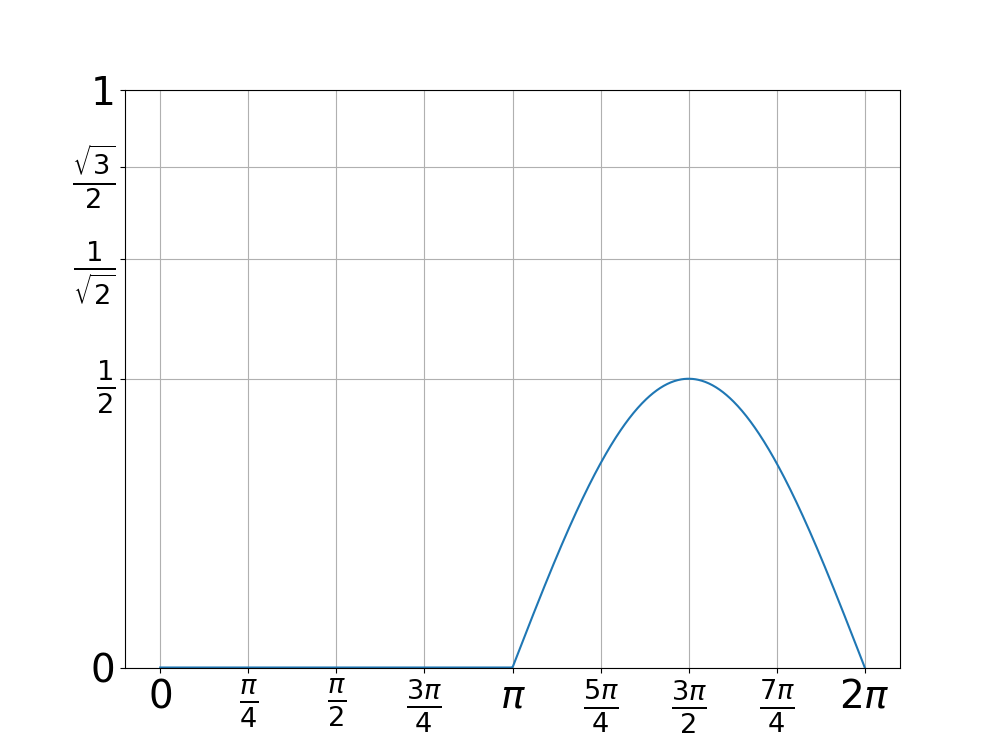
\includegraphics[width=\textwidth]{img/noson/chapter04/section4_1/phi.png}
        \caption{Wave function graph of example state $\ket \varphi$}
        \label{fig:noson-equation-4-5-phi}
    \end{subfigure}
    \caption{Illustrative examples of wave functions graphs.}
    \label{fig:noson-equation-4-5-psi-and-phi}
\end{figure}

As an example, consider the given graphs.
\footnote{The graphs are \emph{merely illustrative}.}
Assume that $\psi(x)$ can also be written as
\begin{align}
    \psi(x) = \begin{cases}
        \frac{sin(x)}{2} &, x \in [0, \pi] \\
        0 &, \text{otherwise}
    \end{cases}.
\end{align}
The graph of $\psi(x)$ is illustrated in
\hyperref[fig:noson-equation-4-5-psi]{Figure \ref{fig:noson-equation-4-5-psi}}.
\hyperref[fig:noson-equation-4-5-psi]{Figure \ref{fig:noson-equation-4-5-phi}}
illustrates the function $\varphi(x)$ assumed as
\begin{align}
    \varphi(x) = \begin{cases}
        \frac{sin(x - \pi)}{2} &, x \in (\pi, 2\pi] \\
        0 &, \text{otherwise}
    \end{cases}.
\end{align}
Additionally, let $\psi^*(x)$ denote the complex conjugate of $\psi(x)$,
that is, $\psi^*(x) = \braket \psi x$.
In the given example, $\psi^*(x) = \psi(x)$ an $\varphi^*(x) = \varphi(x)$.
Note that $\ket \psi$ and $\ket \varphi$ are orthogonal.
\begin{align}
	\braket \psi \varphi &= \int dx \braket \psi x \braket x \varphi \\
	&= \int \psi^*(x) \varphi(x)\ dx \\
	&= \int \psi(x) \varphi(x)\ dx \\
	&= \int 0\ dx \\
	&= 0
\end{align}

\begin{figure}[htb]
    \centering
    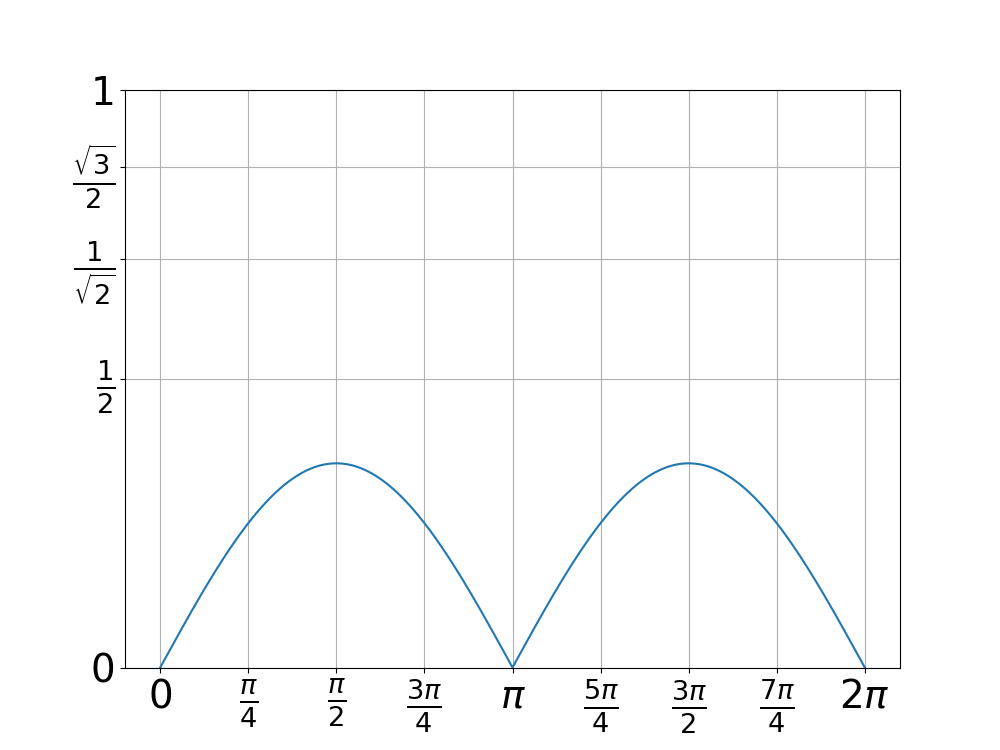
\includegraphics[width=0.45\textwidth]{img/noson/chapter04/section4_1/mu.png}
    \caption{Wave function graph of example state $\ket \mu$}
    \label{fig:noson-equation-4-5-mu}
\end{figure}

Therefore, it is possible to write another state $\ket \mu$ as
a linear compination of $\ket \psi$ and $\ket \varphi$.
The camel hump
\footnote{\href{https://twitter.com/GustavowlKoruja/status/1100581409008336897}{
    There is a good reason to mention camels.}
}
graph in
\hyperref[fig:noson-equation-4-5-psi]{Figure \ref{fig:noson-equation-4-5-mu}}
represents the superposition state
$\ket\mu = \frac{1}{\sqrt2} \ket\psi + \frac{1}{\sqrt2} \ket\varphi$.

Analogously to Equation (4.5),
the probability of obtaining state $\ket{\psi}$ after measuring
$\ket \mu$ can be calculated by
\begin{align}
    p(\psi) &= \frac{|c_i|^2}{\sum_j |c_j|^2} \\[5pt]
    &= \frac{|\braket{\psi}{\mu}|^2}{\braket \mu \mu} \\[5pt]
    &= \frac{|\int dx \braket \psi x \braket x \mu|^2}{\int dx \braket \mu x \braket x \mu} \\[5pt]
    &= \frac{|\int \psi(x) \mu(x)\ dx|^2}{\int \mu(x)^2\ dx} \\
    &= \frac{|\int_0^\pi \psi(x) \mu(x)\ dx + \int_\pi^{2\pi} \psi(x) \mu(x)\ dx|^2}{1^2} \\
    &= \left| \frac{1}{\sqrt2} + 0 \right|^2 \\
    &= \frac 1 2.
\end{align}
Which matches $|\frac{1}{\sqrt2}|^2$,
as defined by the Quantum Mechanics postulates.

\begin{figure}[htb]
    \centering
    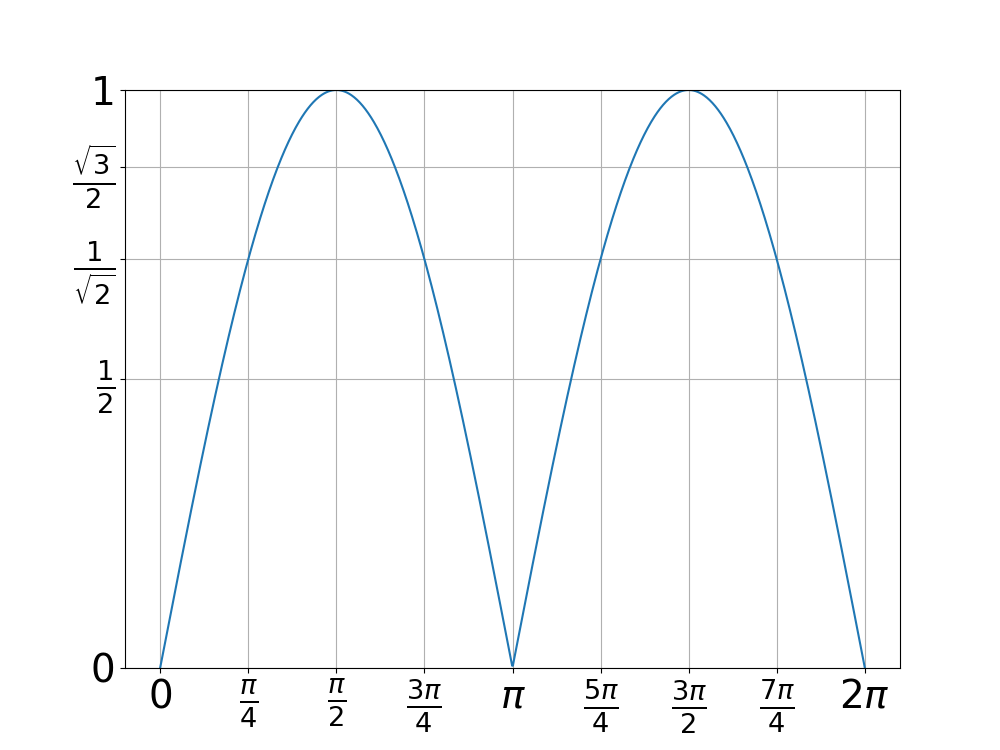
\includegraphics[width=0.45\textwidth]{img/noson/chapter04/section4_1/2-sqrt2-mu.png}
    \captionsetup{width=0.9\textwidth}
    \caption{Graph of state $\ket \mu$ multiplied  by $2 \sqrt2$.
        The amplitudes of $\ket \mu$ are increased,
        but the proportion is maintained.}
    \label{fig:noson-equation-4-5-2-sqrt2-mu}
\end{figure}

If $\ket\mu$ is multiplied by a complex number, $2 \sqrt 2$ for example,
then the graph
\hyperref[fig:noson-equation-4-5-2-sqrt2-mu]{Figure \ref{fig:noson-equation-4-5-2-sqrt2-mu}}
is obtained.
The "new" $\ket{\mu'}$ is now described by
$\ket{\mu'} = 2 \sqrt2 \ket \mu = 2 \ket \psi + 2 \ket \varphi$.
However, by calculating $p(\psi)$, the previous result is also obtained ($\frac 1 2$),
\begin{align}
    p(\psi) = &= \frac{|\braket{\psi}{\mu'}|^2}{\braket{\mu'}{\mu'}} \\[5pt]
    &= \frac{|2 \sqrt2 \braket{\psi}{\mu}|^2}{( (2 \sqrt2)^* \bra \mu)\ (2 \sqrt2 \ket \mu)} \\[5pt]
    &= \frac{|2 \sqrt2|^2 |\braket{\psi}{\mu}|^2}{|2 \sqrt2|^2 \braket{\mu}{\mu}} \\[5pt]
    &= \frac{|\int dx \braket \psi x \braket x \mu|^2}{\int dx \braket \mu x \braket x \mu} \\[5pt]
    &= \frac 1 2 .
\end{align}

\begin{figure}[htb]
    \centering
    \begin{subfigure}[t]{0.45\textwidth}
        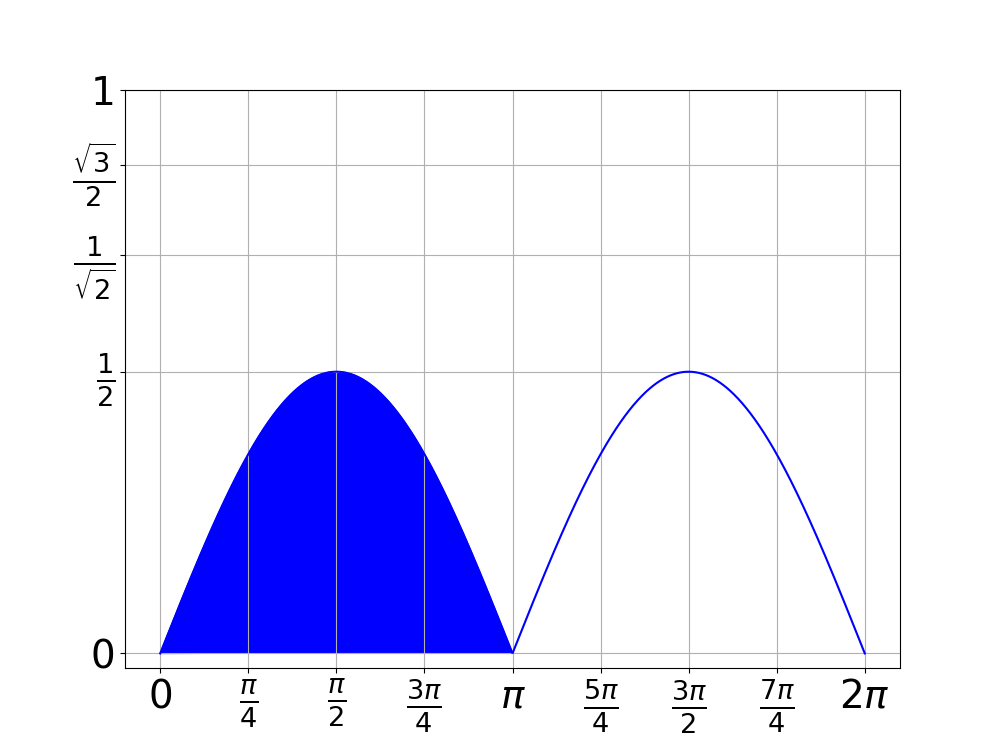
\includegraphics[width=\textwidth]{img/noson/chapter04/section4_1/measure-psi-from-mu.png}
        \captionsetup{width=0.9\textwidth}
        \caption{The probability of $\ket \mu$ collapsing to $\ket \psi$ is
            highlighted in the blue area.}
        \label{fig:noson-equation-4-5-measurement-mu}
    \end{subfigure}
    \begin{subfigure}[t]{0.45\textwidth}
        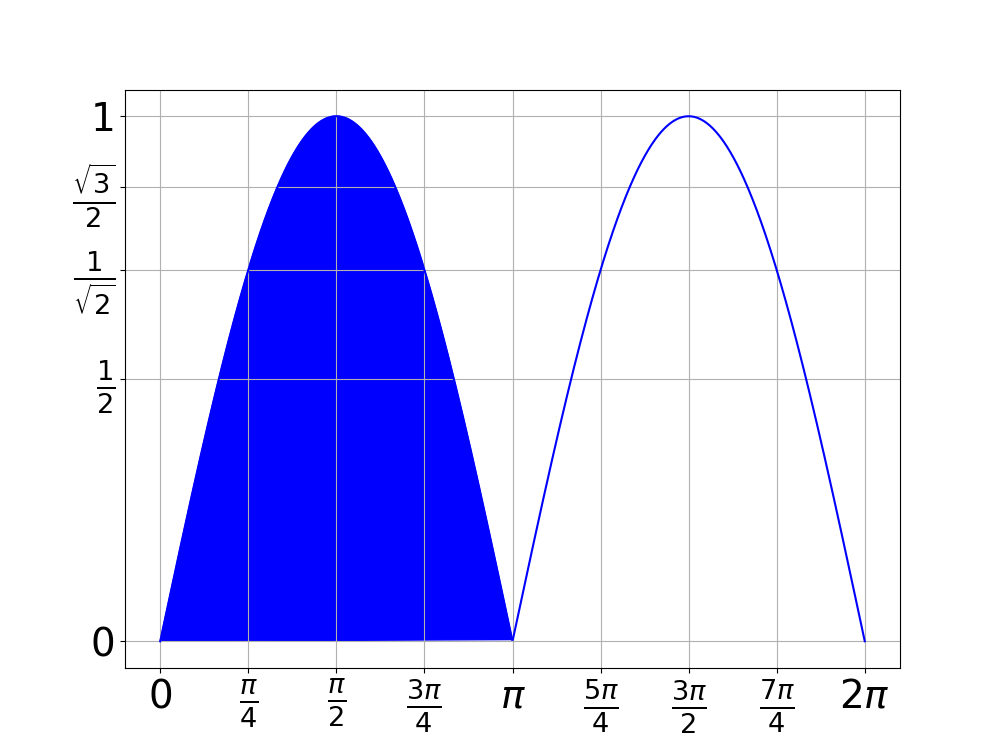
\includegraphics[width=\textwidth]{img/noson/chapter04/section4_1/measure-psi-from-2-sqrt2-mu.png}
        \captionsetup{width=0.9\textwidth}
        \caption{The probability of $2 \sqrt 2 \ket \mu$ collapsing to $2 \sqrt 2 \ket \psi$ is
            highlighted in the blue area.}
        \label{fig:noson-equation-4-5-measurement-2-sqrt2-mu}
    \end{subfigure}
    \captionsetup{width=0.9\textwidth}
    \caption{Both images highlight the part of $\ket \mu$ that corresponds to $\ket \psi$.
        Note that the proportion between the highlighted and non-highlighted areas is preserved,
        even if $\ket \mu$ is multiplied by any complex constant.
        Figures \ref{fig:noson-equation-4-5-measurement-mu} and
        \ref{fig:noson-equation-4-5-measurement-2-sqrt2-mu}
        illustrate the wave function of
        $\ket \mu$ and $2 \sqrt2 \ket \mu$, respectively.}
    \label{fig:noson-equation-4-5-measurement-probabilities}
\end{figure}

By comparing these equations,
it is possible to conclude that
the probabilities are \emph{proportional} to graph area.
This result can be visualised in
\hyperref[fig:noson-equation-4-5-measurement-probabilities]{
    Figure \ref{fig:noson-equation-4-5-measurement-probabilities}
}
It is more accurate, however, to assert that
the probability of measuring $\ket i$ is \emph{proportional}
to its projection on $\ket \psi = \sum_i c_i \ket i$,
i.e. $P(i) \propto |\braket i \psi |^2$.
Which corresponds exactly to Postulate III of Quantum Mechanics as stated by
Shankar's \href{https://www.springer.com/br/book/9780306447907}{Principles of Quantum Mechanics}.